% Chapter 5
\label{Capítulo5}
\chapter{Resultados}
\begin{center}
    \textit{``Newton's third law. You've got to leave something behind''}
     
     Cooper
\end{center}
Os testes foram realizados com o objetivo de validar a implementação do \acrshort{lare} e verificar se os resultados obtidos correspondem aos esperados. A confrontação dos resultados experimentais foi efetuada com recurso ao \href{https://www.multisim.com}{\textit{MultisimLive}}, ao \textit{VirtualBench} e aos valores teóricos previamente descritos na Secção \ref{sec:experiencias}. Para a análise dos resultados, serão apresentados um ou dois exemplos representativos por tipo de experiência, sendo que os restantes são obtidos de forma análoga.

No caso específico da Lei de \textit{Ohm}\footnote{Uma vez que a versão grátis \textit{online} do \textit{MultisimLive} não permite realizar a análise continua - \textit{dc sweep} - esta análise fez-se utilizando o \href{https://www.circuitlab.com/}{CircuitLab}}, há ainda a possibilidade de verificar os valores com recurso a um multímetro de bancada.

As experiências podem ser realizadas com diferentes combinações e configurações:
\begin{itemize}
	\item \textbf{Lei de \textit{Ohm}}: três opções de estudo de resistências;
	\item \textbf{Rectificadores}: quatro combinações possíveis de resistências e condensadores para cada rectificador;
	\item \textbf{Filtros}: duas combinações possiveis de resistências e condensadores para cada filtro.
\end{itemize}

\section{Lei de \textit{Ohm}}
\label{sec:resultados_lei_de_ohm}
O objetivo desta experiência é determinar o valor de uma determinada resistência através do cálculo do declive da recta obtida no gráfico da tensão em função da corrente e, assim, confirmar a Lei de \textit{Ohm}. A Figura \ref{fig:graphohmrepetido}, que novamente aqui se apresenta, representa o gráfico esperado. \textbf{NOTA: Vale a pena? é correcto? Opinião PROF}

\begin{figure}[hbtp]
	\centering
	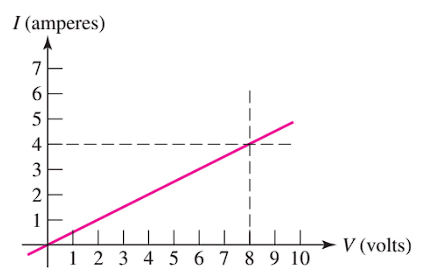
\includegraphics[width=0.3\textwidth]{figures/grafico_Ohm.png}
	\caption{Gráfico da Lei de \textit{Ohm}}
	\label{fig:graphohmrepetido}
\end{figure}

\subsection{Resultados experimentais}
\label{sec:resultados_praticosOHM}
No \acrshort{lare} o utilizador efectua cinco medições de cada grandeza (tensão e corrente), para uma das três resistências disponíveis.

Na Figura \ref{fig:resultados_medicoes_1k} está representado o resultado de um par de medições para uma resistência de \SI{1}{\kilo\ohm}. As restantes medições, em intervalos de \SI{1}{\volt} até \SI{5}{\volt}, são obtidas de forma análoga.

\begin{figure}[hbtp]
	\centering
	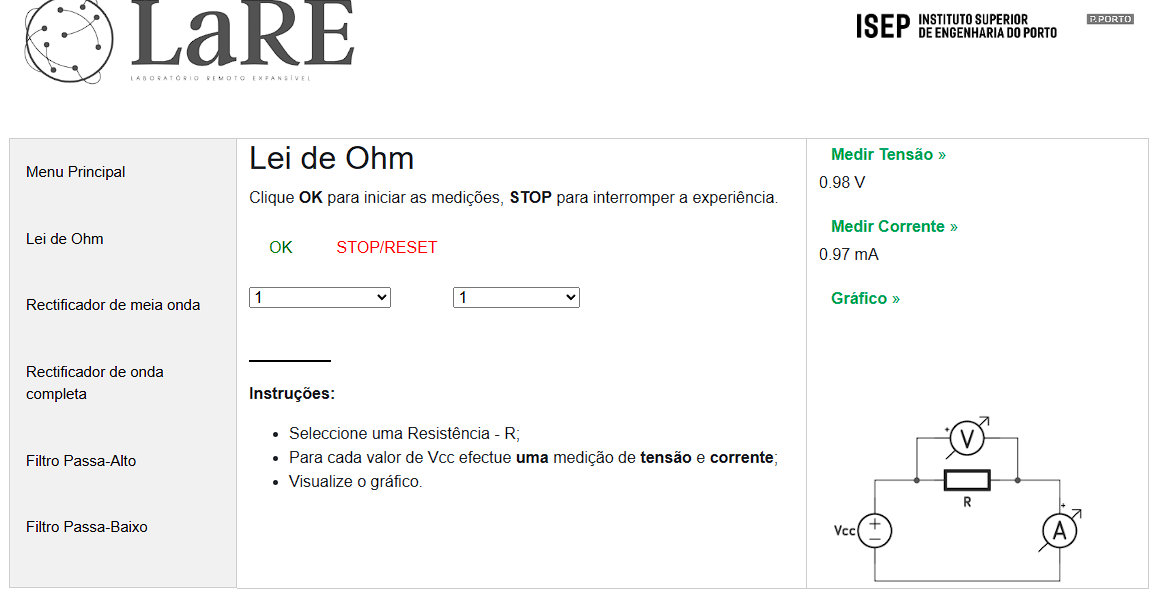
\includegraphics[width=0.7\textwidth]{figures/resultados_medicoes_ohm.png}
	\caption{Medição práctica}
	\label{fig:resultados_medicoes_1k}
\end{figure}

O valor real da resistência, obtida por medição directa, é de \SI{998}{\ohm}, estando dentro da tolerância que é de $\pm$5\%.

O erro associado aos instrumentos de medição pode ser considerado desprezável. De acordo com as especificações do modelo \textit{VB-8012}\cite{datasheetvb8012}, a precisão para medições de tensão em corrente contínua é:

\begin{itemize}
	\item Faixa de \SI{1}{\volt}
	\begin{itemize}
		\item Precisão garantida (1 ano): $\pm$(0.015\% da leitura $\pm$ 0.005\% da faixa)
	\end{itemize}
\end{itemize}

Estes valores indicam que, para uma leitura de \SI{1}{\volt}, o erro máximo estimado devido à precisão do instrumento seria de, aproximadamente $\pm$\SI{0.0002}{\volt}, ou seja, $\pm$\SI{0.2}{\milli\volt}.

Portanto, a diferença entre a tensão fornecida pela fonte — \SI{1}{\volt} — e os valores medidos — \SI{0.98}{\volt} e \SI{0.97}{\milli\ampere} — deve-se, principalmente, à tolerância da resistência utilizada. Assim, conclui-se que os valores medidos se encontram dentro dos limites expectáveis, sendo perfeitamente aceitáveis face às tolerâncias envolvidas.

O gráfico \textit{U vs I}, obtido para esta resistência é apresentado na Figura \ref{fig:grafico_LaRE_1k}. O declive da recta, que representa a resistência, foi calculado e confrontado com o valor real da resistência. 

\begin{figure}[hbtp]
	\centering
	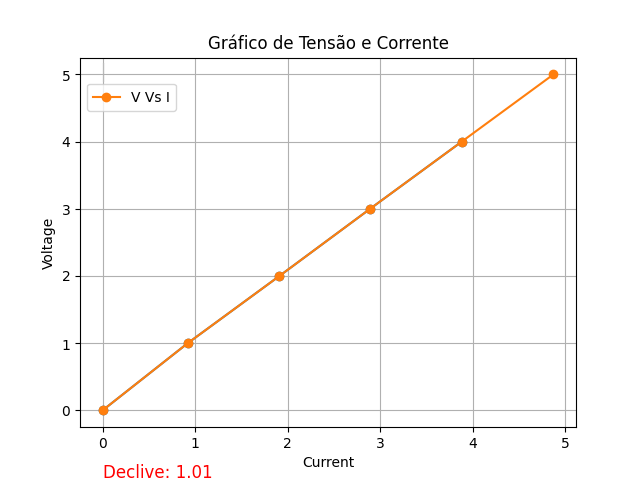
\includegraphics[width=0.7\textwidth]{figures/ohm_graph.png}
	\caption{Gráfico da Lei de \textit{Ohm} - \SI{1}{\kilo\ohm} - MUDAR}
	\label{fig:grafico_LaRE_1k}
\end{figure}

O erro relativo entre o valor teórico(real) e o valor obtido experimentalmente, pode ser calculado através da Equação \ref{eq:errorelativo}:

\begin{equation} \label{eq:errorelativo}
	\text{Erro Relativo} = \frac{|R_{real} - R_{obtido}|}{R_{real}} \times 100
\end{equation}

No caso descrito em cima, o erro relativo obtido é de, aproximadamente, \SI{1.2}{\percent}, sendo um valor perfeitamente aceitável.

Ainda assim e como forma de complementar a análise dos resultados, foram efectuados testes complementares usando dois simuladores, neste caso, o \href{https://www.multisim.com}{\textit{MultisimLive}} e o \href{https://www.circuitlab.com/}{\textit{CircuitLab}}. A Figura \ref{fig:multisimOHM} e a Figura \ref{fig:circuitlab} mostram os resultados obtidos.

\begin{figure}[hbtp]
	\centering%
		\centering
		\subfloat[\centering Multisim\label{fig:multisimOHM}]{{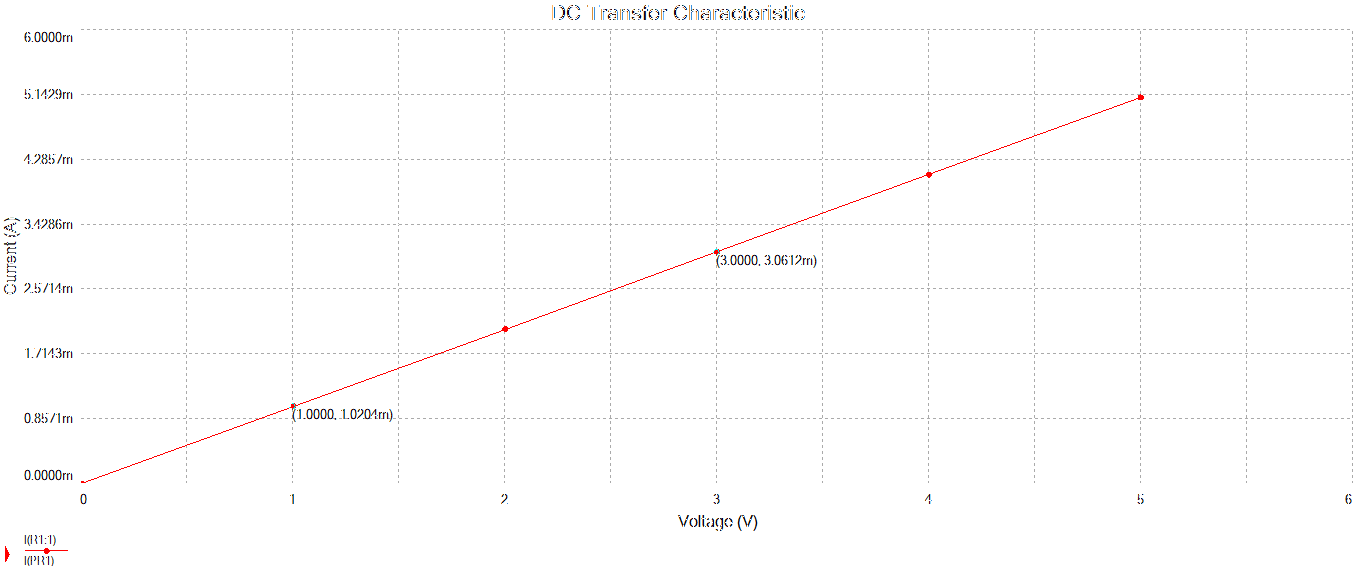
\includegraphics[width=6.3cm]{figures/OHM_resultado_multisim.png} }}%
		\qquad
		\subfloat[\centering CircuitLab\label{fig:circuitlab}]{{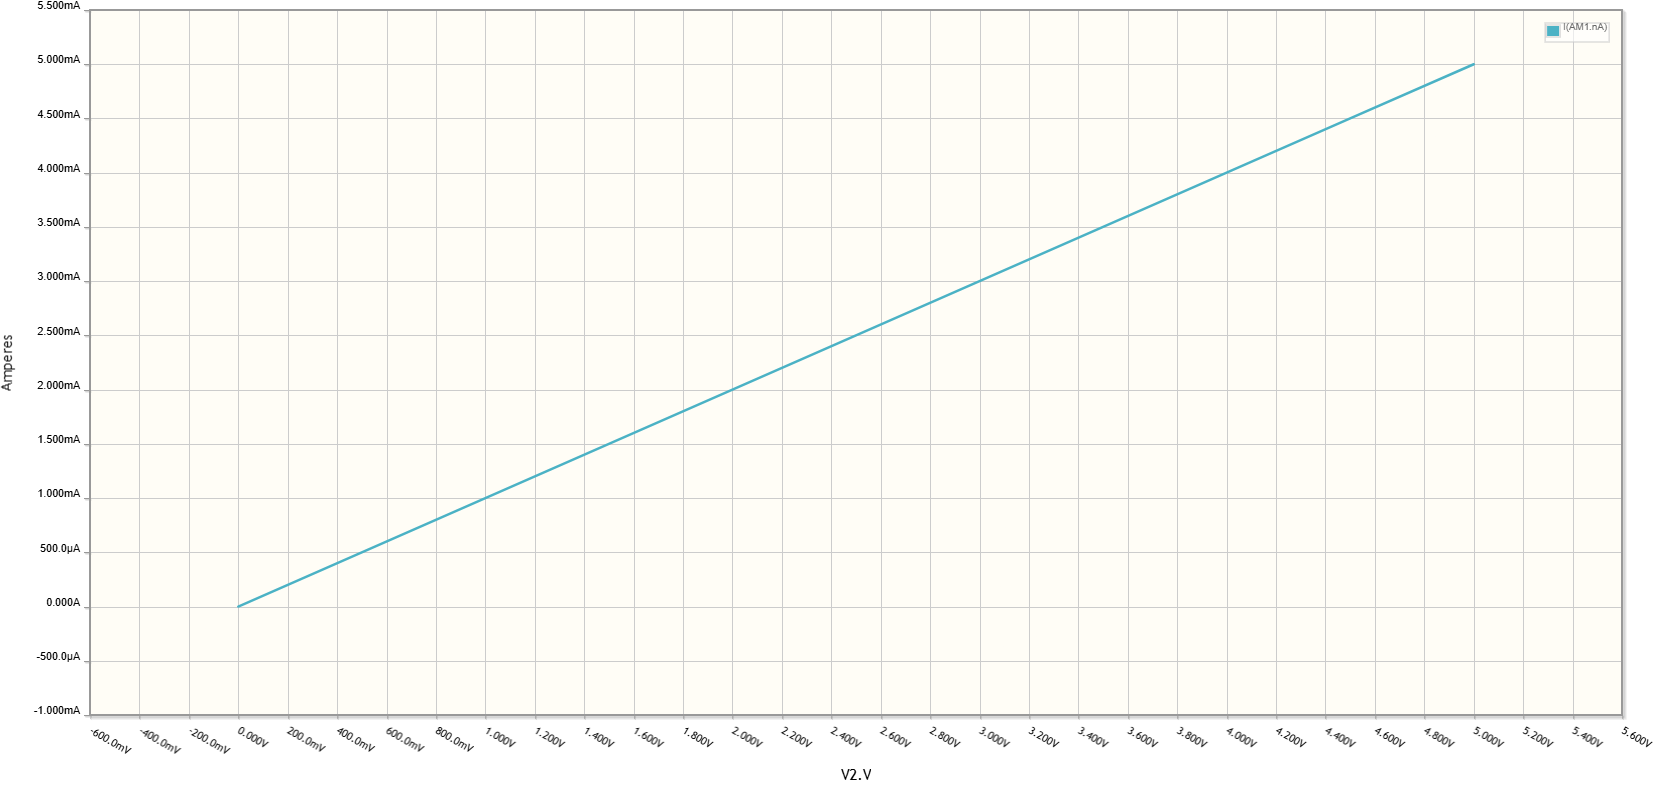
\includegraphics[width=6.3cm]{figures/OHM_resultado_circuitlab.png} }}%
		\caption{Experiência Lei de \textit{Ohm}}%
		\label{fig:experienciaOHM_simuladores}%
	\end{figure}

Através da análise do gráfico obtido no \textit{MultisimLive} e no \textit{CircuitLab} é possível calcular os declives das rectas, dados pela Equação \ref{eq:declive}

\begin{equation} \label{eq:declive}
	\text{m} = \frac{y_{b} - y_{a}}{x_{b} - x_{a}}
\end{equation}

O valor do declive, correspondente à resistência, obtido para estes dois simuladores é, respectivamente, $m_\text{{multisim}} \approx{0.980}$ e $m_{\text{CircuitLab}} \approx{1.002}$. Tendo em conta que a escala do eixo do $y$ está representada em \SI{}{\milli\ampere}, os valores das resistências surgem expressos em \SI{}{\kilo\ohm}, isto é, $R_\text{{multisim}} = \SI{0.980}{\kilo\ohm}$ e $R_{\text{CircuitLab}} = \SI{1.002}{\kilo\ohm}$.  Assim aplicando a Equação~\ref{eq:errorelativo} obtém-se um erro relativo de \SI{1.80}{\percent} e \SI{0.4}{\percent}, respectivamente.

Pela análise dos gráficos obtidos, conclui-se que os resultados obtidos com o \acrshort{lare} são semelhantes aos obtidos com os simuladores e aos valores reais.

\textbf{NOTA PROF: Vale a pena fazer o gráfico com um circuito real?}

\section{Rectificadores}
\label{sec:resultados_rectificadores}
As duas experiências foram implementados com o objectivo de estudar e avaliar a tensão de \textit{ripple} nos circuitos rectificadores de meia onda e onda completa, considerando as quatro combinações possíveis dos pares resistência/condensador. COLOCAR REFERÊNCIA.

As formas de onda esperadas estão representadas na Figura \ref{fig:sedraripple} e Figura \ref{fig:sedraripplecompleta} sendo os valores teóricos da tensão de \textit{ripple} determinados pela Equação \ref{eq:vripplecompleta} e Equação \ref{eq:vrippleOC} - (ou Equação \ref{eq:vripple}). \textbf{NOTA: Aqui coloquei a referência às imagens, ao contrário da Lei de ohm. Opinião PROF}

\subsection{Resultados experimentais [meia onda]}
\label{sec:resultados_RectificadoresMeiaOnda}
Nestas experiências implementadas no \acrshort{lare} os utilizadores podem escolher uma das quatro combinações de resistência e condensador, fazer variar a frequência entre \SI{50}{\hertz} e \SI{2000}{\hertz} e analisar a diferença de valores na tensão de \textit{ripple}.

Sendo assim, a análise será feita para o caso em que $f=\SI{200}{\hertz}$, $R=\SI{2.2}{\kilo\ohm}$ e $C=\SI{4.7}{\micro\farad}$. Para se determinar qual expressão a usar para calcular a tensão de \textit{ripple}, é necessário verificar a condição descrita na Equação \ref{eq:verificarcondicao}:

\begin{equation} \label{eq:verificarcondicao}
	\SI{2.2}{\kilo\ohm} * \SI{4.7}{\micro\farad} >> \dfrac{1}{200}
\end{equation}

Uma vez que esta condição não se verifica, a expressão a utilizar para calcular a tensão de \textit{ripple} teórica é dada pela Equação \ref{eq:vripplecompleta}. O resultado obtido está representado na Equação \ref{eq:vripplecalculado}:

\begin{equation} \label{eq:vripplecalculado}
	U_{r} = \SI{5}{\volt}(1-e^{-\frac{\SI{0.005}{\second}}{\SI{2.2}{\kilo\ohm}*\SI{4.7}{\micro\farad}}}) \approx \SI{1.92}{\volt}
\end{equation}

\textbf{NOTA: Falta a análise aos resultados experimentais do LaRE. Tenho os gráficos mas preciso de colocar os valores máximos para depois calcular o erro.}

Os resultados obtidos experimentalmente usando o circuito real, estão representados na Figura \ref{fig:ripplerealmeiaonda}.

\begin{figure}[hbtp]
	\centering
	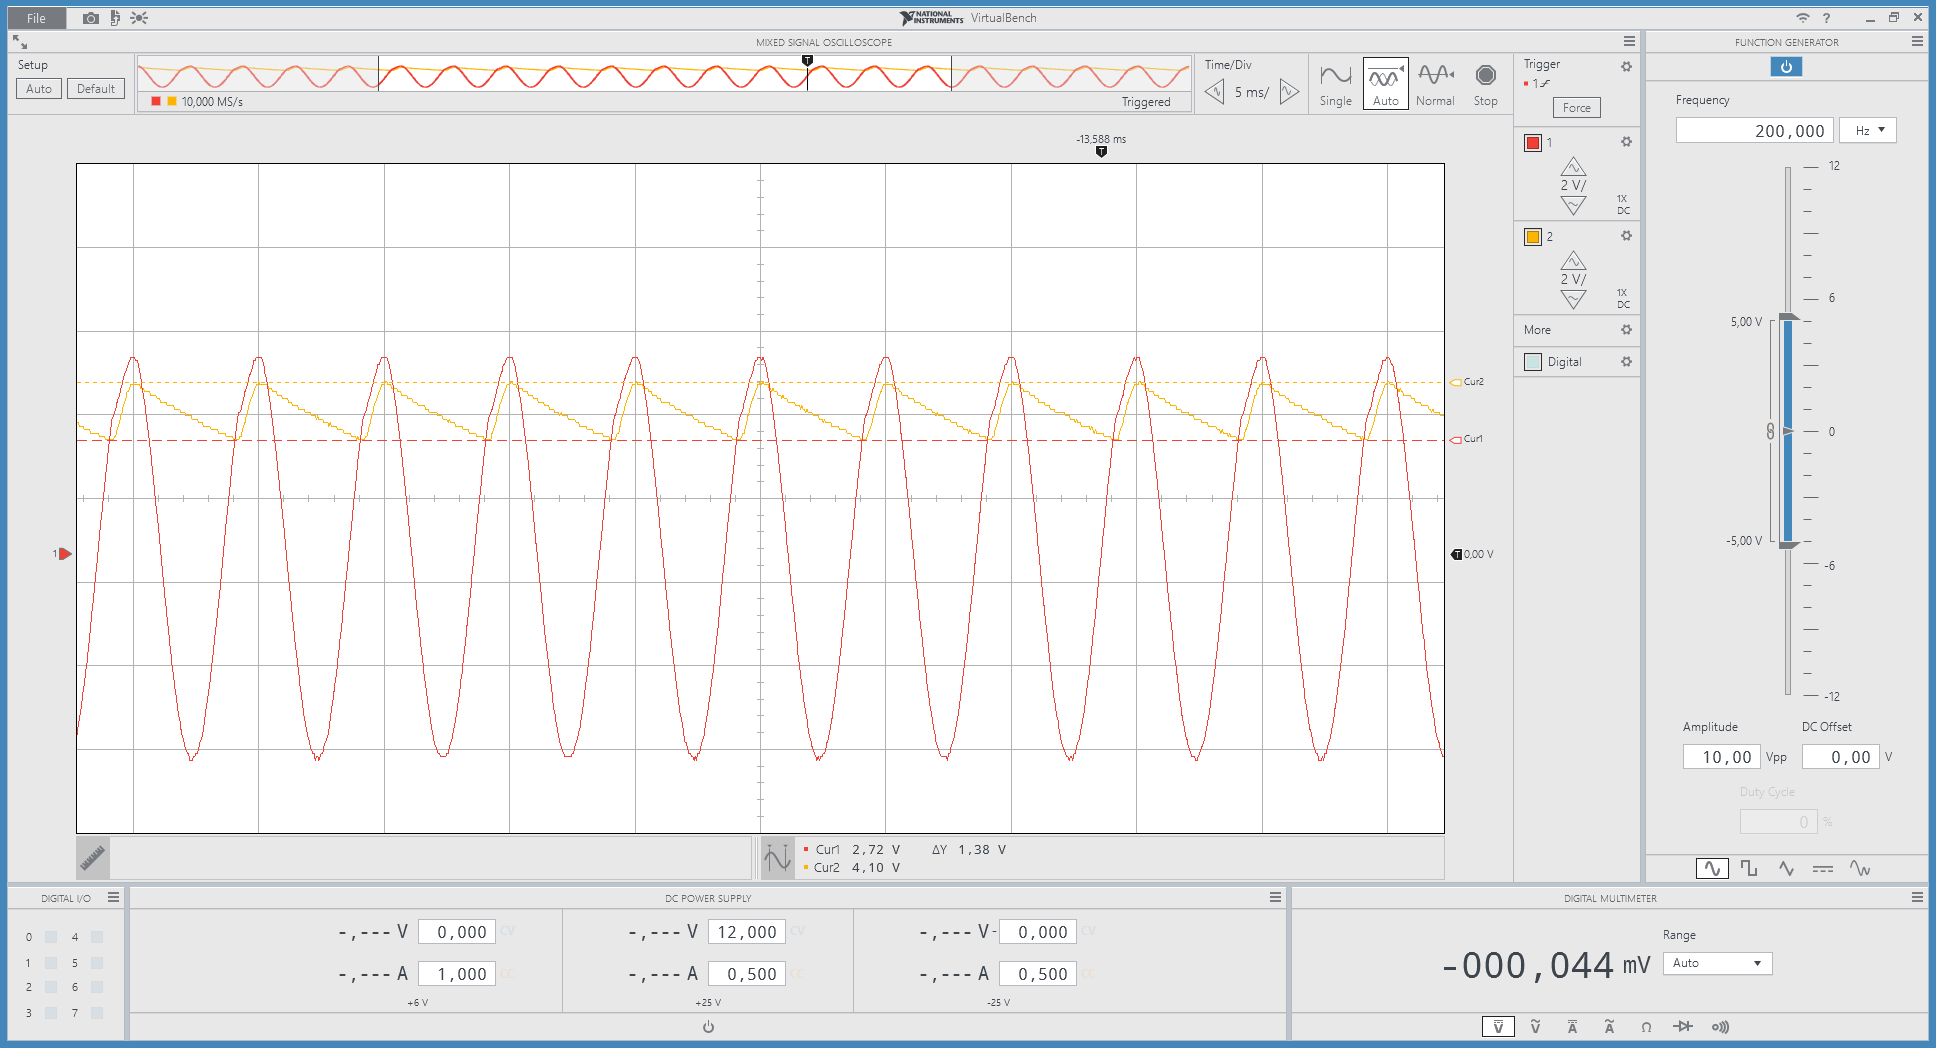
\includegraphics[width=0.7\textwidth]{figures/meiaonda-4.7-2.2.png}
	\caption{Tensão de \textit{ripple} experimental - meia onda - circuito real}
	\label{fig:ripplerealmeiaonda}
\end{figure}

O valor obtido foi de: \SI{1.38}{\volt}, representado na figura pelo $\Delta y$.

Para complementar os resultados experimentais, foi também realizada uma simulação no \textit{Multisim}. Os valores obtidos, bem como a respetiva forma de onda, encontram-se representados na Figura \ref{fig:rippleexperimentalmeiaonda}.

\begin{figure}[hbtp]
	\centering
	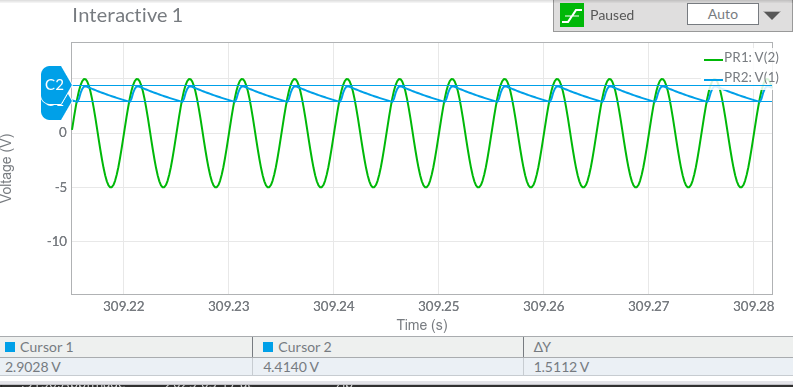
\includegraphics[width=0.7\textwidth]{figures/resultados_meia-onda.png}
	\caption{Tensão de \textit{ripple} experimental - meia onda - 	\textit{multisim}}
	\label{fig:rippleexperimentalmeiaonda}
\end{figure}

A tensão de \textit{ripple} obtida é de, aproximadamente, \SI{1.51}{\volt}, representado novamente pelo $\Delta y$.

\textbf{NOTA PROF: Vale a pena incluir outra análise com o circuitlab? Enretanto, actualizo as imagens com o esquema do circuito.}

Os erros relativos obtidos foram de \SI{28.13}{\percent} e \SI{21.35}{\percent}, respetivamente para os valores medidos experimentalmente e simulados no Multisim. Esta diferença em relação ao valor calculado teoricamente deve-se a diversos fatores, entre os quais se destaca a simplificação inerente à expressão analítica utilizada, que assume componentes ideais e condições perfeitas — como uma resistência constante e um condensador sem perdas \cite{sedrasmith}. A simulação, embora mais próxima da realidade, utiliza também componentes ideais por omissão, como é o caso do condensador sem resistência série (ESR). Ainda assim, considera fenómenos como as quedas de tensão nos díodos e os efeitos transitórios do circuito. A maior discrepância nos valores experimentais pode ser justificada por erros de leitura e pelas elevadas tolerâncias típicas dos condensadores electrolíticos. Assim, as diferenças observadas são compreensíveis e enquadram-se dentro do esperado.

\subsection{Resultados experimentais [onda completa]}
\label{sec:resultados_RectificadoresOndacompleta}

\section{Filtros}
\label{sec:resultados_filtros}
Estas duas experiências foram realizadas com o objetivo de estudar a resposta em frequência dos filtros $RC$, nomeadamente nas configurações passa-alto e passa-baixo, resultantes das diferentes configurações entre as resistências e os condensadores. Os utilizadores podem variar a frequência entre \SI{50}{\hertz} e \SI{80000}{\hertz}, analisando o comportamento da tensão de saída em função da frequência. A frequência de corte é calculada através da Equação \ref{eq:frequenciacorte}, sendo posteriormente comparada com os valores obtidos experimentalmente no diagrama de \textit{Bode}. Adicionalmente, a atenuação da tensão de saída pode ser determinada através da Equação \ref{eq:relacaoGanho}, ou expressa em \SI{}{\decibel} utilizando a Equação \ref{eq:relacaoGanhodB}.

\subsection{Resultados experimentais [filtro passa-alto]}
\label{sec:resultados_filtros_passaalto}
O circuito analisado será o filtro passa-alto, representado na Figura \ref{fig:filtro_pa} e configurado com $R=\SI{2.2}{\kilo\ohm}$ e $C=\SI{10}{\nano\farad}$. Os gráficos que se esperam obter estão representados na Figura \ref{fig:Bode_pa} e Figura{}. Para os restantes valores e configurações, os resultados poderão obtidos de forma análoga.

Para estes valores, a frequência de corte teórica é dada pela Equação \ref{eq:frequenciacorte}, sendo que o valor obtido é de \SI{7234.32}{\hertz}.

Os valores experimentais obtidos com o \acrshort{lare} estão representados na Figura \ref{fig:voutvinlare}. Como se pode ver pela análise da figura, o ganho a altas frequências é prácticamente unitário.

\begin{figure}[hbtp]
	\centering
	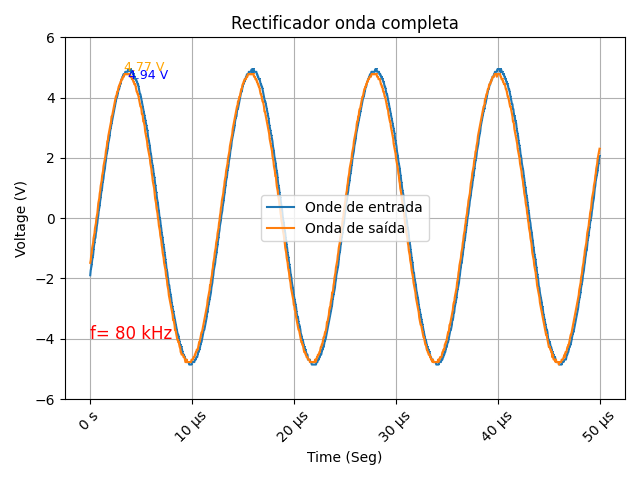
\includegraphics[width=0.7\textwidth]{figures/filtro_passa-alto.png}
	\caption{$v_{out}$ \textit{vs} $v_{in}$ experimental \acrshort{lare} - TEMPORÁRIO}
	\label{fig:voutvinlare}
\end{figure}

Comparando estes valores com os obtidos através do circuito real, representados na Figura \ref{fig:realPA} e Figura \ref{fig:multisimPA} do circuito simulado no \textit{multisim} verifica-se que os valores obtidos são prácticamente iguais, podendo ser considerado, com segurança, que em ambos os casos o ganho de tensão é unitário. \textbf{NOTA: Podem ficar duas imagens separadas. Opinião PRof}

\textbf{NOTA: Dado o avançado da hora e o cansaço, não fiz o gráfico para a fc no lare. Acrescento na pr´xoma versão. No entanto, tenhos os gráficos prontos para fazer a análise do diagrama de Bode}

\begin{figure}[hbtp]
	\centering%
		\centering
		\subfloat[\centering Circuito real\label{fig:realPA}]{{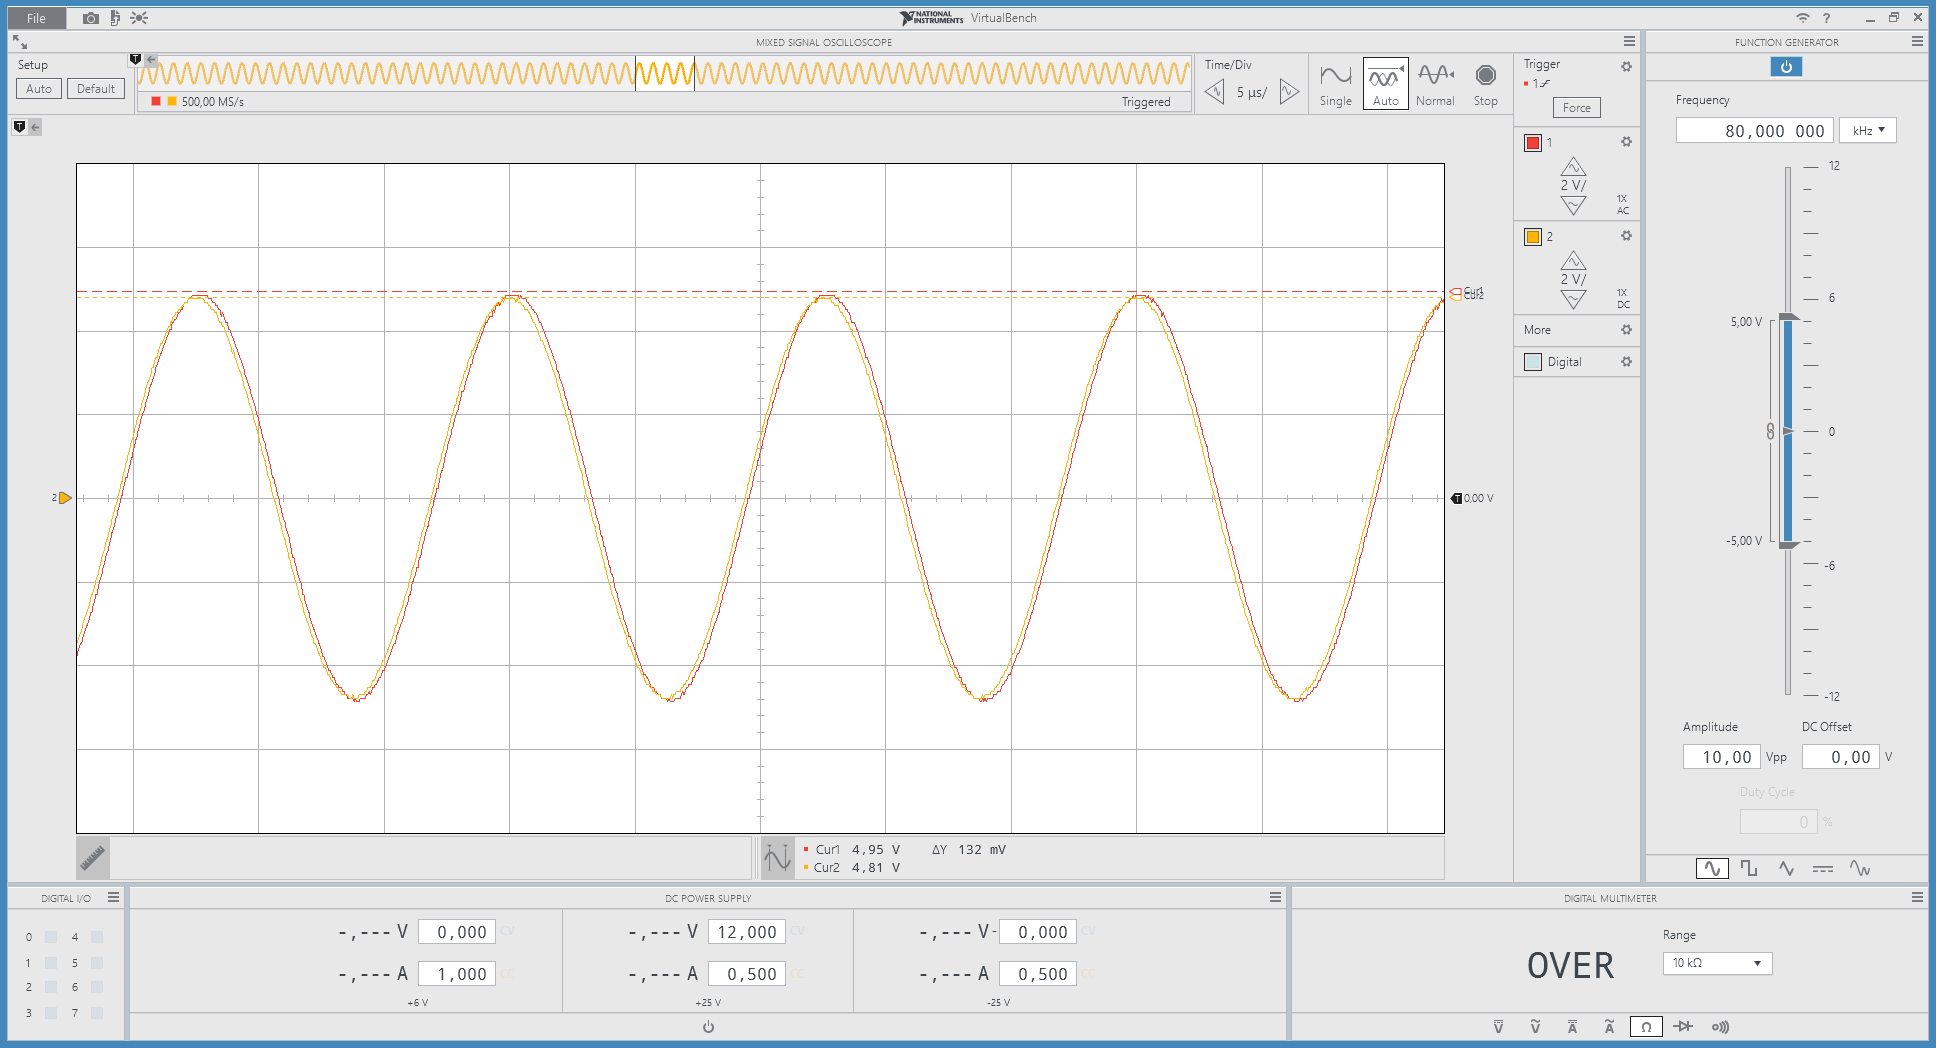
\includegraphics[width=6.3cm]{figures/PA_10nF2k2-80Khz.png} }}%
		\qquad
		\subfloat[\centering simulação \textit{multisim}\label{fig:multisimPA}]{{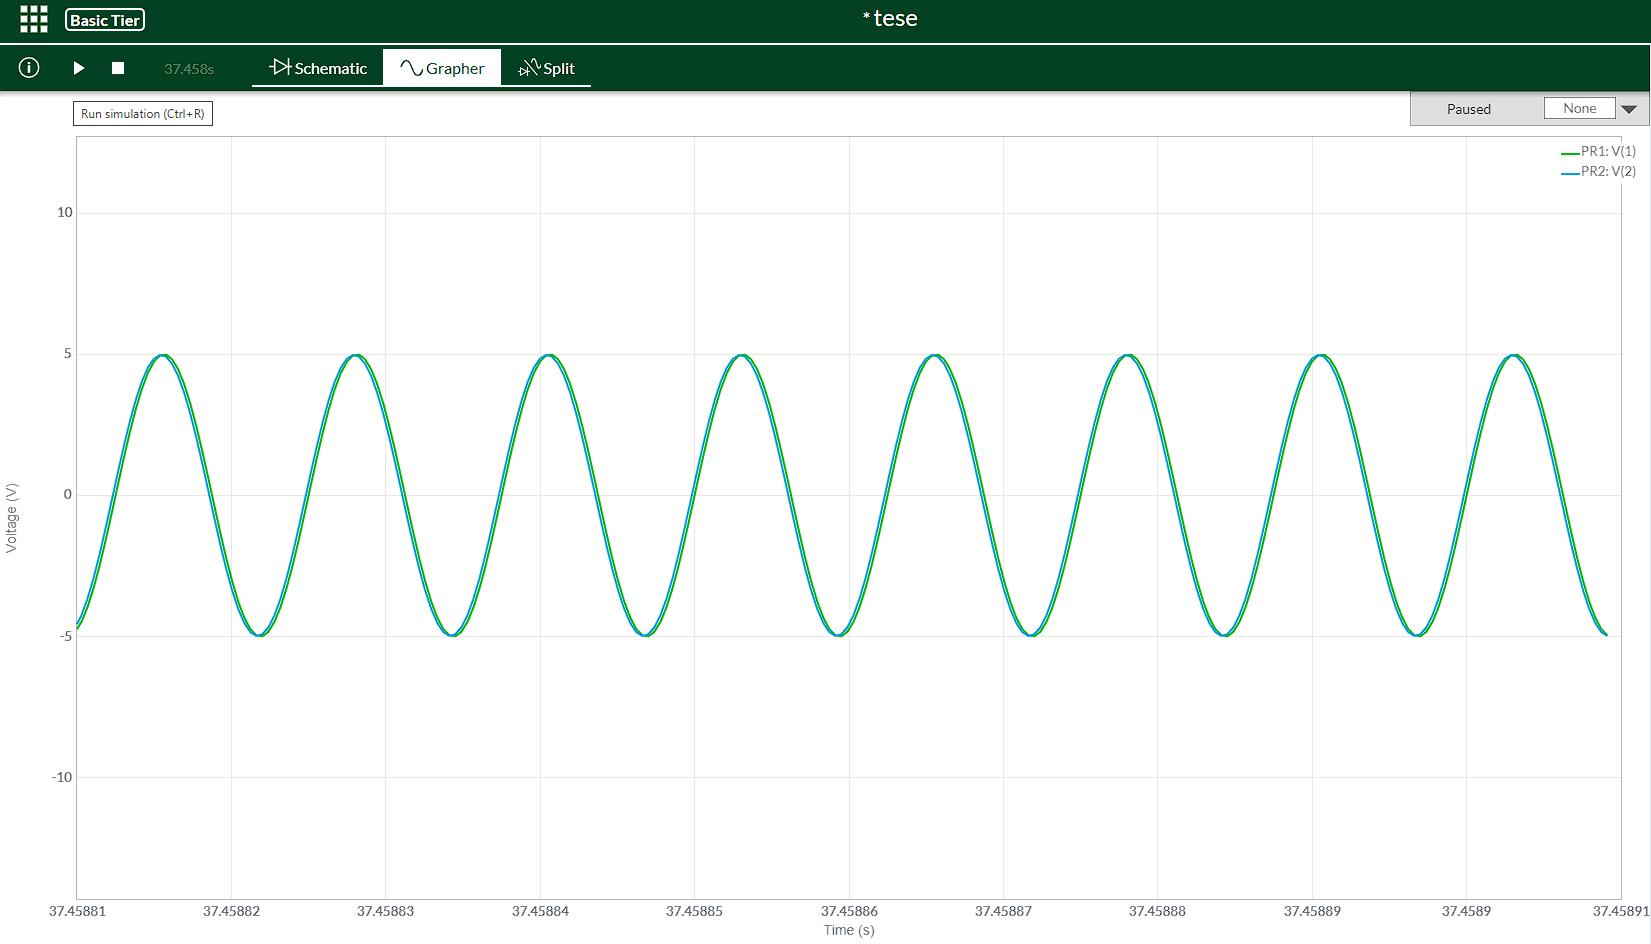
\includegraphics[width=6.3cm]{figures/boda_HPF_vout.png} }}%
		\caption{Valores experimentais reais e simulados - $v_{out}$ \textit{vs} $v_{in}$}%
		\label{fig:simulacaoPA}%
	\end{figure}

Relativamente à análise ao digarama de \textit{Bode}, pode ver-se na Figura \ref{fig:fcBode} que o valor aproximado da frequência de corte, obtido no \acrshort{lare}, é de \SI{7071.1}{\hertz}. O erro relativo é, aproximadamente, \SI{2.26}{\percent}. Este valor é perfeitamente aceitável, tendo em conta a tolerância dos componentes utilizados, os erros de medição e aproximações.

\begin{figure}[hbtp]
	\centering
	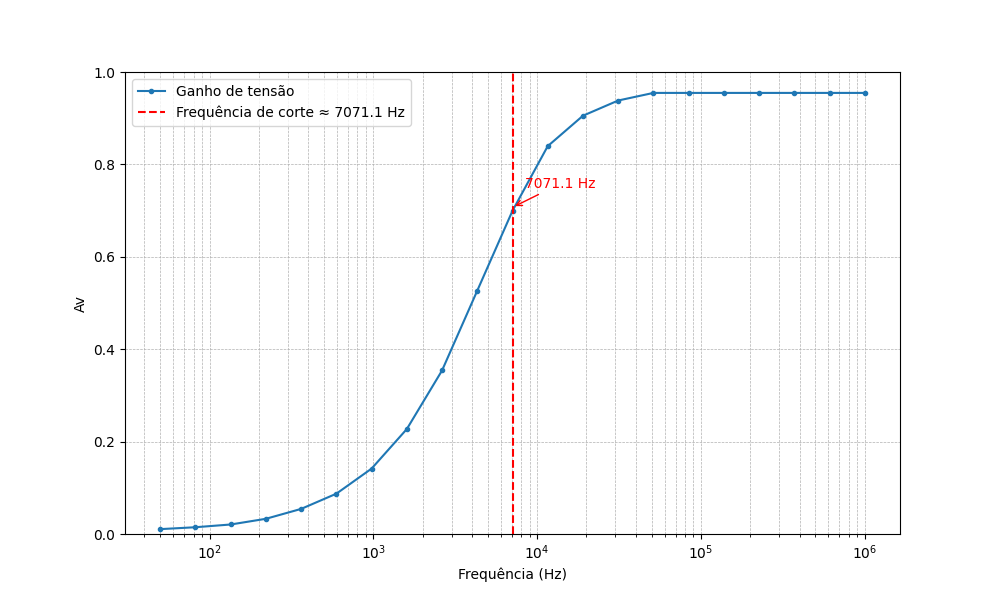
\includegraphics[width=0.7\textwidth]{figures/bode_hpf_fc.png}
	\caption{Frequência de corte - filtro passa-alto - Diagrama de \textit{Bode}}
	\label{fig:fcBode}
\end{figure}

Os resultados complementares obtidos com base na simulação efectuada no \textit{multisim}, já que o \acrshort{virtualbench} não permite gerar o diagrama de Bode, representados na Figura \ref{fig:fcBodemultisim}, mostram que a frequência de corte é de \SI{7282.4}{\hertz}. O erro relativo é de \SI{0.67}{\percent}, o que é prácticamente desprezável.

\begin{figure}[hbtp]
	\centering
	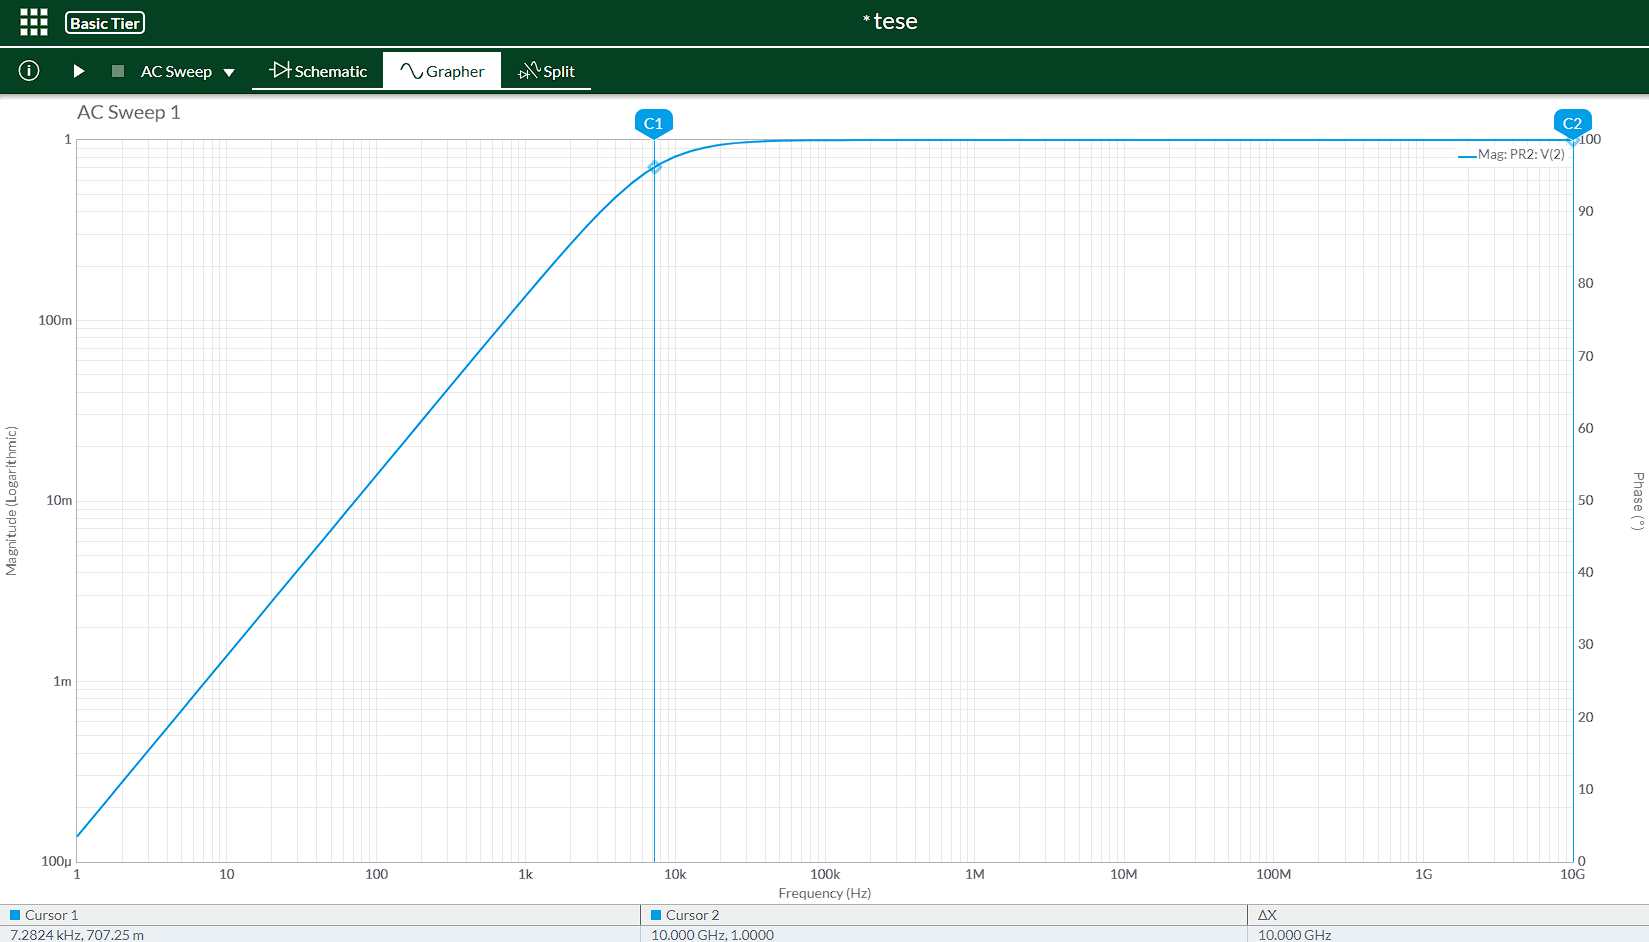
\includegraphics[width=0.7\textwidth]{figures/boda_HPF_fc.png}
	\caption{Frequência de corte - \textit{multisim} - Diagrama de \textit{Bode}}
	\label{fig:fcBodemultisim}
\end{figure}

\section{Limitações}
\section{Melhoramentos}


